\documentclass[a4paper,12pt]{article}
%\documentclass[a4paper,12pt]{scrartcl}

\usepackage{xltxtra}

\input{../preamble.tex}



\usepackage[spanish]{babel}

% \setromanfont[Mapping=tex-text]{Linux Libertine O}
% \setsansfont[Mapping=tex-text]{DejaVu Sans}
% \setmonofont[Mapping=tex-text]{DejaVu Sans Mono}

\title{Redes Petri}
\author{Isaac Ayala Lozano}
\date{2020-03-05}

\begin{document}
\maketitle

\section{Problema}
Sea la secuencia de
funcionamiento expresada en el
diagrama de movimientos, de un
dispositivo con modalidad de ciclo
continuo con inicio y paro del ciclo.

\begin{figure}[htb!]
\centering
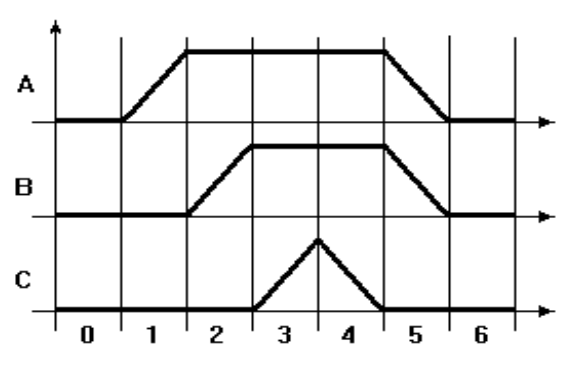
\includegraphics[width=0.5\textwidth]{hw02_sequence.png}
 \caption{Secuencia de funcionamiento.}
\end{figure}


En este caso se consideran tres actuadores con cilindros neumáticos
denominado A, B y C,
Respectivamente se asocian sensores de finales de carrera:
$a_0$, $a_1$, $b_0$, $b_1$, $ c_0 $ y $ c_1$.
Se incluyen los comandos de inicio de ciclo y paro de ciclo.
Del diagrama de movimientos, se obtiene la secuencia $A_1, $$ B_1$, $ C_1$, $ C_0 $ y $ A_0-B_0$.

\section{Solución}

Se presenta la red Petri en la Figura \ref{fig: PN}.

\begin{figure}[htb!]
\import{img/}{hw02_PN.pdf_tex}
 \caption{Red Petri.}
 \label{fig: PN}
\end{figure}




\begin{itemize}
 \item Ecuaciones de inscripción
 \begin{align}
  K_0 &= \text{Stop} \land a_1 \land b_1 \land Q_5 \\
  K_1 &= (\text{Start} \land Q_0) \lor (Q_5 \land a_1 \land b_1 \land \lnot \text{Stop})\\
  K_2 &= Q_1 \land a_0\\
  K_3 &= Q_2 \land b_0\\
  K_4 &= Q_3 \land c_0\\
  K_5 &= Q_4 \land c_1
 \end{align}

%
\item Ecuaciones de borrado
\begin{align}
 J_0 &= Q_1\\
 J_1 &= Q_2\\
 J_2 &= Q_3\\
 J_3 &= Q_4\\
 J_4 &= Q_5\\
 J_5 &= Q_0 \lor Q_1
\end{align}
%
\item Ecuaciones de salida
\begin{align}
 A_0 &= Q_1\\
 B_0 &= Q_2\\
 C_0 &= Q_3\\
 C_1 &= Q_4\\
 A_1 &= Q_5\\
 B_1 &= Q_5
\end{align}

\end{itemize}




% \printbibliography

\end{document}
